\documentclass[12pt]{article}
\usepackage{latexsym,amssymb,amsmath} % for \Box, \mathbb, split, etc.
% \usepackage[]{showkeys} % shows label names
\usepackage{cite} % sorts citation numbers appropriately
\usepackage{path}
\usepackage{url}
\usepackage{verbatim}
\usepackage{graphicx}
\usepackage{array}
\usepackage{multirow}

% horizontal margins: 1.0 + 6.5 + 1.0 = 8.5
\setlength{\oddsidemargin}{0.0in}
\setlength{\textwidth}{6.5in}
% vertical margins: 1.0 + 9.0 + 1.0 = 11.0
\setlength{\topmargin}{0.0in}
\setlength{\headheight}{12pt}
\setlength{\headsep}{13pt}
\setlength{\textheight}{625pt}
\setlength{\footskip}{24pt}

\renewcommand{\textfraction}{0.10}
\renewcommand{\topfraction}{0.85}
\renewcommand{\bottomfraction}{0.85}
\renewcommand{\floatpagefraction}{0.90}
\usepackage{graphicx}
\usepackage{wrapfig}
\usepackage{lscape}
\usepackage{rotating}
\usepackage{epstopdf}
\makeatletter
\setlength{\arraycolsep}{2\p@} % make spaces around "=" in eqnarray smaller
\makeatother

% change equation, table, figure numbers to be counted inside a section:
\numberwithin{equation}{section}
\numberwithin{table}{section}
\numberwithin{figure}{section}

% begin of personal macros
\newcommand{\half}{{\textstyle \frac{1}{2}}}
\newcommand{\eps}{\varepsilon}
\newcommand{\myth}{\vartheta}
\newcommand{\myphi}{\varphi}
\usepackage[utf8]{inputenc}

% Default fixed font does not support bold face
\DeclareFixedFont{\ttb}{T1}{txtt}{bx}{n}{8} % for bold
\DeclareFixedFont{\ttm}{T1}{txtt}{m}{n}{8}  % for normal

% Custom colors
\usepackage{color}
\definecolor{deepblue}{rgb}{0,0,0.5}
\definecolor{deepred}{rgb}{0.6,0,0}
\definecolor{deepgreen}{rgb}{0,0.5,0}
\definecolor{backcolour}{rgb}{0.96,0.96,0.96}

\usepackage{listings}

% cpp style for highlighting
\newcommand\cppstyle{\lstset{
		language=C++,
        basicstyle=\tiny\ttfamily,
		keywordstyle=\color{blue}\ttfamily,
		stringstyle=\color{red}\ttfamily,
		commentstyle=\color{green}\ttfamily,
		morecomment=[l][\color{magenta}]{\#},
		frame=tb,                         % Any extra options here
showstringspaces=false,            % 
backgroundcolor=\color{backcolour}
}}


% cpp environment
\lstnewenvironment{cpp}[1][]
{
	\cppstyle
	\lstset{#1}
}
{}

% cpp for external files
\newcommand\cppexternal[2][]{{
		\cppstyle
		\lstinputlisting[#1]{#2}}}

% cpp for inline
\newcommand\cppinline[1]{{\cppstyle\lstinline!#1!}}

\newcommand{\IN}{\mathbb{N}}
\newcommand{\IZ}{\mathbb{Z}}
\newcommand{\IQ}{\mathbb{Q}}
\newcommand{\IR}{\mathbb{R}}
\newcommand{\IC}{\mathbb{C}}
\newcommand{\Real}[1]{\mathrm{Re}\left({#1}\right)}
\newcommand{\Imag}[1]{\mathrm{Im}\left({#1}\right)}
\usepackage{booktabs}
\usepackage{caption}
\usepackage{float}
\usepackage{titlesec}
\usepackage{capt-of}
%dashed line
\usepackage{array}
\usepackage{arydshln}
\setlength\dashlinedash{0.2pt}
\setlength\dashlinegap{1.5pt}
\setlength\arrayrulewidth{0.3pt}

%Widows & Orphans & Penalties

\widowpenalty500
\clubpenalty500
\clubpenalty=9996
\exhyphenpenalty=50 %for line-breaking at an explicit hyphen
\brokenpenalty=4991
\predisplaypenalty=10000
\postdisplaypenalty=1549
\displaywidowpenalty=1602
\floatingpenalty = 20000
\usepackage[T1]{fontenc}
\usepackage{fontspec}
\setmainfont[Scale=0.85, Ligatures={Required,Common,Contextual,TeX}]{TeX Gyre Schola} % Incredible font inside latex


\newcommand{\norm}[2]{\|{#1}\|_{{}_{#2}}}
\newcommand{\abs}[1]{\left|{#1}\right|}
\newcommand{\ip}[2]{\left\langle {#1}, {#2} \right\rangle}
\newcommand{\der}[2]{\frac{\partial {#1}}{\partial {#2}}}
\newcommand{\dder}[2]{\frac{\partial^2 {#1}}{\partial {#2}^2}}
\usepackage{enumitem}
\newcommand{\nn}{\mathbf{n}}
\newcommand{\xx}{\mathbf{x}}
\newcommand{\uu}{\mathbf{u}}
\usepackage{tikz}
\usetikzlibrary{arrows}
\usetikzlibrary{positioning}
\usepackage{titlesec}
\newcommand{\junk}[1]{{}}
\usepackage{sectsty}
\usepackage{xcolor}

\newcommand\MyBox[2]{
	\fbox{\lower0.75cm
		\vbox to 1.7cm{\vfil
			\hbox to 1.7cm{\hfil\parbox{1.4cm}{#1\\#2}\hfil}
			\vfil}%
	}%
}

\makeatletter
\renewcommand*\env@matrix[1][\arraystretch]{%
	\edef\arraystretch{#1}%
	\hskip -\arraycolsep
	\let\@ifnextchar\new@ifnextchar
	\array{*\c@MaxMatrixCols c}}
\makeatother

\makeatletter
\renewcommand*\env@matrix[1][*\c@MaxMatrixCols c]{%
	\hskip -\arraycolsep
	\let\@ifnextchar\new@ifnextchar
	\array{#1}}
\makeatother

\definecolor{darkblue}{rgb}{0,0,0.4}
\usepackage[colorlinks = true,
linkcolor = darkblue,
urlcolor  = darkblue,
citecolor = darkblue,
anchorcolor = darkblue]{hyperref}
% set two lengths for the includegraphics commands used to import the plots:
\newlength{\fwtwo} \setlength{\fwtwo}{0.45\textwidth}
% end of personal macros

\begin{document}
\DeclareGraphicsExtensions{.jpg}

\begin{center}
\textsc{\Huge Multi-core Programming} \\[2pt]
	\textsc{\Large Assignment 2}\\
	\vspace{0.5cm}
  Ali Gholami \\[6pt]
  Department of Computer Engineering \& Information Technology\\
  Amirkabir University of Technology  \\[6pt]
  \def\UrlFont{\em}
  \url{https://aligholamee.github.io}\\
\href{mailto:aligholami7596@gmail.com}{\textit{aligholami7596@gmail.com}}
\end{center}

\begin{abstract}
OpenMP is an implementation of multithreading, a method of parallelizing whereby a master thread (a series of instructions executed consecutively) forks a specified number of slave threads and the system divides a task among them. The threads then run concurrently, with the runtime environment allocating threads to different processors. In this assignment, we are going to implement the parallelization of the matrix multiplication.
\end{abstract} 

\subparagraph{Keywords.} \textit{Heterogeneous Programming, OpenMP, C Programming, C++ Programming, Parallelization, Multi-thread Programming.}

\section{Matrix Multiplication}
\subsection{What's the goal?}
In this assignment, we'll be parallelizing the matrix multiplication using \textit{OpenMP}. The goal is to speed up the matrix multiplication by implementing the parallelization in two axis (\textit{1D} \& \textit{2D}). Below the serial code for the matrix multiplication. Sources for this assignment is available in the repository merged with this report.

\begin{cpp}
		void multiply(DataSet dataSet){
			int i, j, k, sum;
			for(i = 0; i < dataSet.n; i++){
				for(j = 0; j < dataSet.p; j++){
					sum = 0;
					for(k = 0; k < dataSet.m; k++){
						sum += dataSet.A[i * dataSet.m + k] * dataSet.B[k * dataSet.p + j];
					}
					dataSet.C[i * dataSet.p + j] = sum;
				}
			}
		}
\end{cpp}

\subsection{1D Parallelization}
The following figures are provided from the problem description by \textit{Dr. Ahmad Siavashi}. Each of the highlighted areas show a job for a thread. Figure 1.1 shows how the multiplication is done by each thread.
\begin{figure}[!h]\centering
	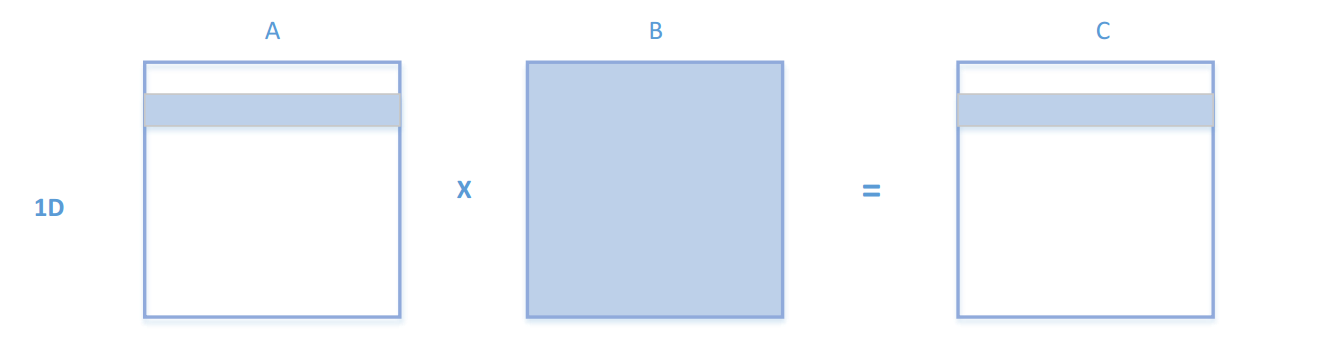
\includegraphics[width=0.9\textwidth]{one_dimensional.png}
	\caption{Matrix Multiplication Parallelization on Horizontal Axis.}
	\label{figsolplot}
\end{figure}\\
Assuming each \textit{integer} as 4 bytes, we'll be filling the table 1.1 using the average time computed after 6 times of running the program. Note that in the dimensions of these matrices is assumed to be same in different axises and we are dealing with squared matrices. According to this assumption, each dimension can be computed as below:
\begin{itemize}
	\item \textbf{100 KB}:  $d = \sqrt{\frac{10^5}{4}} = 158$
	\item \textbf{400 KB}:  $d = \sqrt{\frac{4 * 10^5}{4}} = 316$
	\item \textbf{800 KB}:  $d = \sqrt{\frac{8 * 10^5}{4}} = 447$
	\item \textbf{1 MB}:  $d = \sqrt{\frac{10^{6}}{4}} = 500$
\end{itemize}
\subsubsection{Serial Time}
The average serial time for this multiplication is $0.239668$ seconds.
\subsubsection{Parallelized For Loop}
In order to make things a bit faster, we'll use \textit{pragma} like so:
\begin{cpp}
		void multiply(DataSet dataSet){
			int i, j, k, sum;
			
			#pragma omp parallel for private(i)
			for(i = 0; i < dataSet.n; i++){
				for(j = 0; j < dataSet.p; j++){
					sum = 0;
					for(k = 0; k < dataSet.m; k++){
						sum += dataSet.A[i * dataSet.m + k] * dataSet.B[k * dataSet.p + j];
					}
					dataSet.C[i * dataSet.p + j] = sum;
				}
			}
		}
\end{cpp}

\def\arraystretch{1.3}
\begin{table}[!h]
		\centering
\begin{tabular}{ |p{3cm}||p{2cm}|p{2cm}|p{2cm}|p{2cm}|p{1.5cm}|  }
	
	\hline
	\multicolumn{6}{|c|}{Total Size of Each Matrix} \\
	\hline
	 Num of Threads & 100 KB & 400 KB & 800 KB & 1 MB & Average Speedup\\
	\hline
		1   & 0.024875    & 0.264729 & 0.831792 &   1.115039&   -\\
		2   & 0.025861    & 0.164219 & 0.461315 &   0.653042 &   1.52\\
		4   & 0.030058    & 0.185644 & 0.402523 &   0.562593&   0.97\\
		8   & 0.038876    & 0.273006 & 0.687464 &   0.800365& 0.8\\
	\hline
\end{tabular}
	\caption{Results of 1-Dimensional Parallelization.}
\label{figsolplot}
\end{table}
\newpage
\subsection{2D Parallelization}
The results for the \textit{2D} parallelization is given in the table 1.2.
\begin{figure}[!h]\centering
	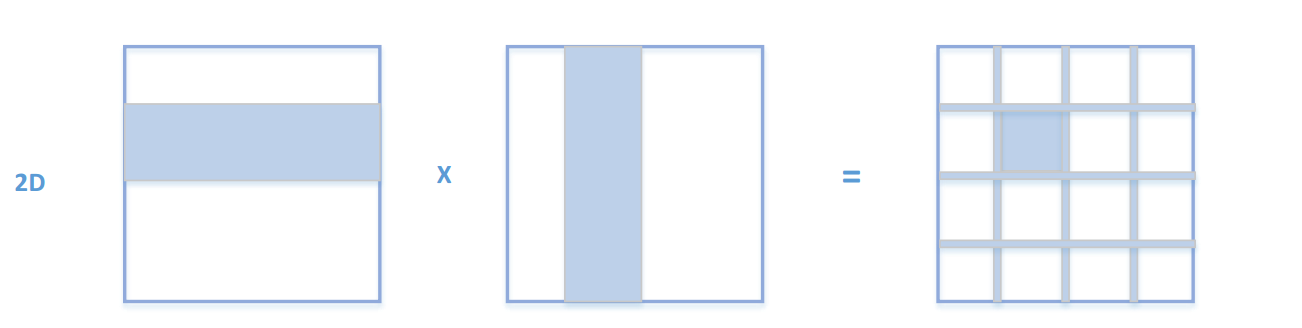
\includegraphics[width=0.9\textwidth]{two_dimensional.png}
	\caption{Matrix Multiplication Parallelization on Horizontal and Vertical Axis.}
	\label{figsolplot}
\end{figure}\\
\subsection{2D Parallelized For Loop}
Each of the threads does the job in the highlighted area.
In order to make things a bit faster, we'll use \textit{pragma} like so:
\begin{cpp}
		void multiply(DataSet dataSet){
			int i, j, k, sum;
			
			#pragma omp parallel for private(i)
			for(i = 0; i < dataSet.n; i++){
				
				#pragma omp parallel for private(j)
				for(j = 0; j < dataSet.p; j++){
					sum = 0;
					for(k = 0; k < dataSet.m; k++){
						sum += dataSet.A[i * dataSet.m + k] * dataSet.B[k * dataSet.p + j];
					}
					dataSet.C[i * dataSet.p + j] = sum;
				}
			}
		}
\end{cpp}

\def\arraystretch{1.3}
\begin{table}
	\centering
	\begin{tabular}{ |p{3cm}||p{2cm}|p{2cm}|p{2cm}|p{2cm}|p{1.5cm}|  }
		
		\hline
		\multicolumn{6}{|c|}{Total Size of Each Matrix} \\
		\hline
	 Num of Threads & 100 KB & 400 KB & 800 KB & 1 MB & Speedup\\
		\hline
		1   & 0.023645 & 0.268649 & 0.839288 & 1.114186 &   -\\
		2   & 0.037867 & 0.165194 & 0.451727 & 0.656459 &   1.4\\
		4   & 0.033289 & 0.203213 & 0.432043 & 0.534328 &   1.045\\
		8   & 0.041303 & 0.271042 & 0.679229 & 0.788940 &   0.7\\
		\hline
	\end{tabular}
	\caption{Results of 2-Dimensional Parallelization.}
	\label{figsolplot}
\end{table}

\end{document}